\chapter{Related Work and Design Space}
\label{chap:design_space}
\label{sec:related-work}

The previous chapter established what graphs are, how they are accessed, and how they are stored.
This chapter surveys the systems that have been built to manage and process graph data, and organizes them into a taxonomy based on three classification features: whether a system operates on property graphs or structural graphs, whether it handles a static snapshot or a dynamic, evolving graph, and whether it provides transactional guarantees for mutations.
We discuss representative systems in each category, highlighting what each provides and what it lacks, and conclude with a distillation of the design space that positions \project{} as a general-purpose system spanning the entire grid.


\section{Property Graphs vs. Structural Graphs}
\label{design:property_vs_structural}
Two features define our overarching characterization of the design space: whether the system manages property graphs or structural graphs and whether the graphs under management are static or dynamic.
Recall that a structural graph results from selections and projections on the labels and properties of an underlying property graph~\cite{RodriguezNeubauer2010}.
One might select edges of a certain type to form a structural graph, for instance, a structural graph of follower relationships in a social network.
The structural graph so constructed ``is homogeneous, composed simply of vertices, edges and, possibly, a weight attached to their elements''~\cite[Section 1]{teseo2021deLeo}.
The structural graph is a useful abstraction for many graph algorithms and queries. It provides a simple graph model that can be used to reason about the graph's structure.
For instance, the structural graph can be used to compute the connectivity of the graph or to compute the influence of a node in the graph.

We assume that the property graph represents ground truth and that the structural graph is derived from the property graph.
A structural graph can be materialized as needed or periodically, as is done at Facebook~\cite{curtiss2013unicorn}.
These materialized structural graphs are essentially snapshots of the property graph at a certain point in time.
We describe these \emph{static structural graphs} in more detail in~\autoref{design:static_structural}.

In contrast, the property graph changes over time.
Since the property graph is the ground truth, the structural graph must stay up-to-date with it.
Two strategies exist: periodic recomputing or incrementally updating as the property graph changes.
The latter produces \emph{dynamic structural graphs}.
We describe dynamic structural graphs in more detail in~\autoref{design:dynamic_structural}.

\project{} stores both the property graph and its derived structural representations in the same transactional \wt{} store.
\textbf{Structural graphs are not separate materialized snapshots that must be rebuilt or shipped to a different engine; they are persistent layouts maintained alongside the property data.}
Switching between property queries and structural analytics therefore requires no data movement.

\autoref{fig:design_space} provides an overview of the design space of structural graphs; the following sections discuss each region in detail.
\begin{figure}[h]
    \centering
    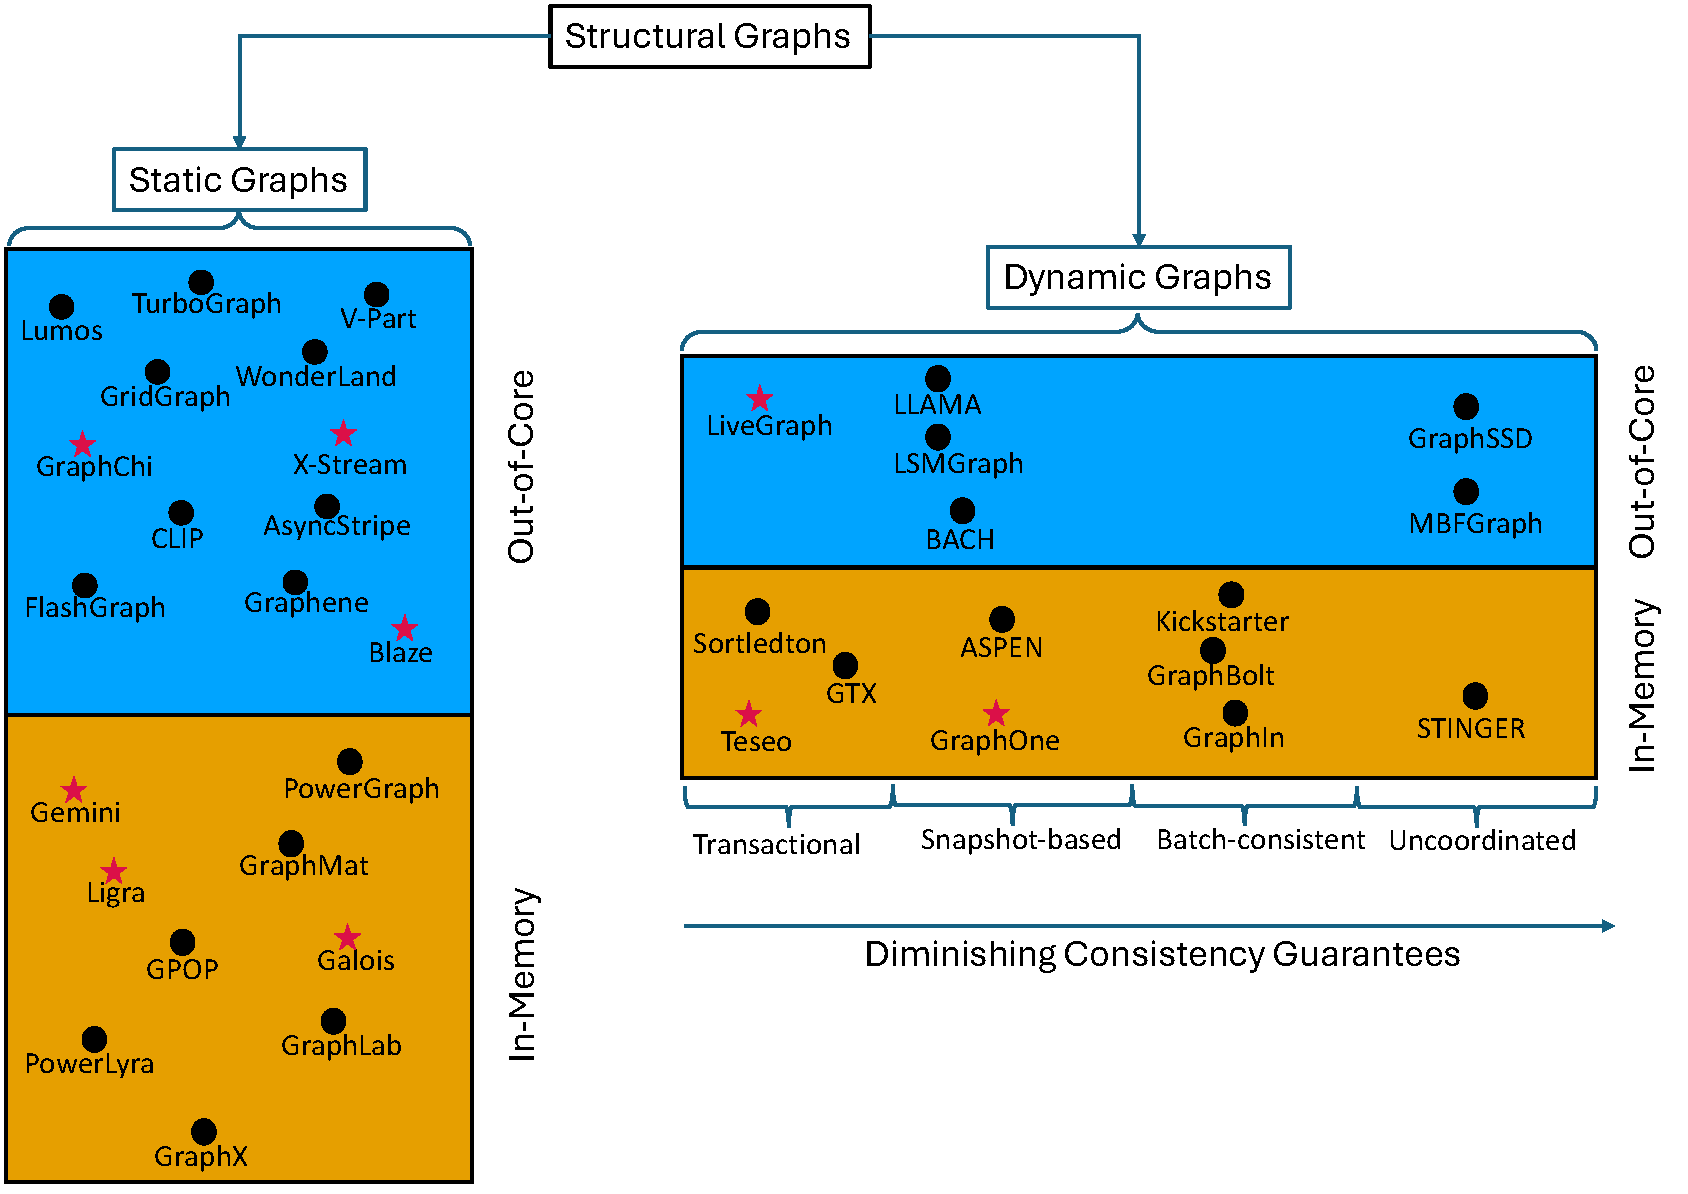
\includegraphics[width=\textwidth]{fig/background/final_taxonomy_struc_new.pdf}
    \caption{Design Space of Graph Data Management Systems handling structural graphs. We compare \project{} to systems marked with {\color[RGB]{219,16,72}\raisebox{-0.1ex}{\scalebox{1.3}{$\star$}}}}
    \label{fig:design_space}
\end{figure}

\section{Static Graph Processing Systems}
\label{design:static_structural}

Static structural graphs have been the main focus of graph processing systems research for over a decade \cite{malewicz2010pregel,gonzalez2014graphx, zhu2016gemini, xing2015petuum, low2012distributed,gonzalez2012powergraph, powerlyra2019,shun2013ligra, nguyen2013lightweight, zhu2016gemini, graphmat, lakhotia2020gpop, beamer2015gap, kim2022blaze, ai2018clip,zheng2015flashgraph}.
These graphs are primarily used for analytics and graph mining tasks focusing on uncovering statistical properties and discovering patterns.
Because these graphs are static, the systems that process them impose no consistency requirement between snapshots.
Each snapshot is produced through a batch \ac{ETL} process and is (often) processed independently of other snapshots.
In a graph database, materializing the structural graph from the property graph constitutes the ``extract'' step.

Once the static \ac{GPS} has a snapshot to process, it must first \emph{preprocess} the graph to construct the data structures needed to execute the graph algorithms.
The preprocessing step reads the graph from an exchange format (often CSV) and builds the data structures needed for storage and processing.
This requires a pass over the graph and can take significantly longer to finish than the analytics task itself (for example, GraphChi takes longer to preprocess the graph than it takes to run Triangle Counting or PageRank).

If the graph data structures obtained after the preprocessing are small enough, they can be stored and processed in memory.
Graph processing systems designed for shared-memory, multi-core machines are usually optimized for in-memory processing.
Several systems have been optimized for this design point: Gemini~\cite{zhu2016gemini}, GraphMat~\cite{graphmat}, Ligra~\cite{shun2013ligra}, Galois~\cite{pingali2011tao}, GPOP~\cite{lakhotia2020gpop}, and GraphLab~\cite{low2012distributed}.
The GAP Benchmark Suite (GAPBS)~\cite{beamer2015gap} provides optimized reference implementations of common analytics kernels on a CSR representation; \project{} adapts these kernels to use its API for a fair comparison.
Ligra~\cite{shun2013ligra} introduces direction-optimizing traversal that switches between sparse and dense modes based on frontier size.
Galois~\cite{nguyen2013lightweight} generalizes graph computation with priority-driven scheduling for irregular parallelism.
Gemini~\cite{zhu2016gemini} uses chunk-based partitioning with locality-aware execution.

If the graph structures are too large to fit in memory on a single machine, they are partitioned across multiple machines.
Examples of distributed graph processing systems include GraphX~\cite{gonzalez2014graphx}, Pregel~\cite{malewicz2010pregel}, PowerGraph~\cite{gonzalez2012powergraph}, Distributed GraphLab~\cite{low2012distributed}, and PowerLyra~\cite{powerlyra2019}.
For the purpose of our taxonomy, we collectively refer to shared-memory, multi-core systems and distributed (in-memory) systems as \textbf{in-memory graph} processing systems.

Over time, researchers noticed that the communication overheads in distributed graph processing systems were high, leading them to underperform when compared to single-threaded systems running on a commodity laptop~\cite{mcsherry2015scalability}.
The need to build systems that can scale to large graphs that do not fit in RAM on a single machine, coupled with the underperformance of distributed graph processing systems, led to the development of out-of-core systems.
These systems cache the most frequently accessed data structures in memory and spill the rest to disk; we call them \textbf{out-of-core graph} processing systems.
The on-disk data layout is designed to maximize sequential I/O and minimize random access to edge data.
Out-of-core systems differ primarily in how they partition edges on disk~\cite{xu2026oocsurvey}.
\emph{Destination-based} systems group edges by destination interval. GraphChi~\cite{kyrola2012graphchi}, the pioneer of out-of-core graph processing, divides vertices into disjoint intervals and constructs one edge shard per interval, processing shards via its Parallel Sliding Windows algorithm.
\emph{Source-based} systems instead group source vertices with their out-edges; TurboGraph~\cite{han2013turbograph} uses this layout to exploit SSD parallelism by issuing concurrent I/O requests across multiple flash channels.
\emph{2-D} partitioning, introduced by GridGraph~\cite{zhu2015gridgraph}, divides the adjacency matrix into a $P \times P$ grid indexed by source and destination intervals, so that the active vertex state for each cell fits in the last-level cache.
X-Stream~\cite{roy2013x} streams an unordered edge list in a scatter-gather model, avoiding any sorted preprocessing altogether.
Blaze~\cite{kim2022blaze} targets NVMe SSDs with partition-centric processing and a lock-free online-binning scheme that saturates device bandwidth.
FlashGraph~\cite{zheng2015flashgraph} takes a semi-external-memory approach, keeping vertex state in RAM and issuing fine-grained asynchronous I/O for edge lists on SSDs.
ChunkGraph~\cite{wang2024chunkgraph} takes a different approach: rather than designing a new computation model, it replaces the OS page cache with a chunk-based graph representation that organizes vertex adjacency lists into degree-classified, variable-size chunks, solving the problem of vertex data spanning page boundaries and improving I/O utilization for power-law graphs.
ChunkGraph works transparently with existing in-memory vertex-centric systems such as Ligra without requiring changes to their computation model.
Other out-of-core systems include CLIP~\cite{ai2018clip}, V-part~\cite{elyasi2019large}, Wonderland~\cite{zhang2018wonderland}, and Mosaic~\cite{maass2017mosaic}; we discuss CLIP's programming model in~\autoref{design:subgraph_centric}.

\autoref{tab:static_systems} summarizes these systems and their key design choices.

\newcommand{\evalstar}{{\color[RGB]{219,16,72}$\star$}}
  \begin{table}[t]
  \centering
  \small
  \begin{tabular}{lll}
  \toprule
  \textbf{Class} & \textbf{System} & \textbf{Key design choice} \\
  \midrule
  \multirow{6}{*}{\rotatebox[origin=c]{90}{In-memory}}
      & GAPBS\evalstar{}          & Optimized reference kernels on CSR \\
      & Ligra\evalstar{}           & Direction-optimizing traversal \\
      & Galois\evalstar{}          & Priority-driven scheduling for irregular parallelism \\
      & Gemini\evalstar{}          & Chunk-based partitioning with locality-aware execution \\
      & GraphMat       & Vertex programs as sparse matrix operations \\
      & GPOP           & Partition-centric processing for cache residency \\
  \midrule
  \multirow{4}{*}{\rotatebox[origin=c]{90}{Distributed}}
      & Pregel         & BSP vertex-centric message passing \\
      & PowerGraph     & GAS decomposition for high-degree vertices \\
      & GraphX         & Graph analytics on Spark RDDs \\
      & PowerLyra      & Hybrid partitioning (high-/low-degree vertices) \\
  \midrule
  \multirow{7}{*}{\rotatebox[origin=c]{90}{Out-of-core}}
      & GraphChi\evalstar{}       & Destination-based shards; Parallel Sliding Windows \\
      & TurboGraph     & Source-based layout; SSD parallelism \\
      & GridGraph      & 2-D grid partitioning; LLC-sized cells \\
      & X-Stream\evalstar{}       & Unordered edge streaming; no sorted preprocessing \\
      & Blaze\evalstar{}          & NVMe-optimized partition-centric processing \\
      & FlashGraph     & Semi-external memory; async I/O for edge lists \\
      & ChunkGraph     & Degree-classified chunks; transparent with Ligra \\
  \bottomrule
  \end{tabular}
  \caption{Summary of static graph processing systems. All require offline preprocessing and support no mutations during processing. \evalstar{} marks systems evaluated against \project{}.}
  \label{tab:static_systems}
  \end{table}

All static systems, whether in-memory or out-of-core, require an offline preprocessing step to build their layout and are batch-only, supporting no mutations during processing.
Among the out-of-core systems we compare to, GraphChi is a partial exception: it includes an evolving-graph mode that can append edges during execution.
Incoming edges are held in per-shard in-memory buffers and periodically flushed to the on-disk shards, triggering shard splits when a shard grows too large.
Shard splits halve computation throughput, and flushes that increasingly compete with computation prevent the mode from sustaining high ingestion rates~\cite{kyrola2012graphchi}.
X-Stream's unordered edge list allows it to absorb batches of new edges that are partitioned and appended to its on-disk stream files via a shared-memory interface, after which algorithms must be recomputed from scratch on the accumulated graph~\cite{roy2013x}.
Blaze offers no dynamic mode.
None of these mechanisms support arbitrary mutations or transactional semantics.
\project{} operates directly on its persistent representation, eliminating the preprocessing step entirely; we include preprocessing time in all comparisons to illustrate this advantage.
\project{} relies on \wt{}'s buffer pool to spill to secondary storage, achieving competitive out-of-core performance without a dedicated I/O framework.
These two classes of graph processing systems constitute a sub-classification of the design space of structural graph data management systems, both static and dynamic (~\autoref{fig:design_space}).

\section{Dynamic Graph Processing Systems}
\label{design:dynamic_structural}
Structural graphs are derived from property graphs, and since the property graph is dynamic, the structural graph must be updated as the property graph changes; this leads to the concept of dynamic structural graphs.
The dynamic nature of these graphs requires some form of consistency.
The system must update the structural graph consistently with the property graph while isolating concurrent queries from in-flight mutations.

The simplest approach is \emph{uncoordinated}: a system applies updates directly to the live graph data structure without creating versions or synchronizing with ongoing queries.
Any concurrent reader may observe a partially applied mutation, which can lead to inconsistent results, query failures, or delayed convergence of iterative algorithms.
STINGER~\cite{stinger2012ediger} is the canonical example: it allows fast concurrent updates via a block-based adjacency list but provides no consistency guarantees.

A more sophisticated approach is \emph{snapshot-based}: the system constructs versioned representations of the graph so that a reader can obtain a consistent point-in-time view.
LLAMA~\cite{llama} achieves this with immutable, copy-on-write CSR layers; ASPEN~\cite{10.1145/3314221.3314598} uses a functional tree (C-tree) with path-copying to create lock-free snapshots.
GraphOne~\cite{graphone2019kumar} uses an append-only edge log paired with an adjacency array and exposes frozen snapshots at a sequence number.
These systems version their read path but do not coordinate writes: GraphOne, for instance, uses blind-write semantics with no conflict detection, and LLAMA uses per-node spinlocks to prevent structural corruption but provides no mechanism for detecting semantic write-write conflicts.

A third approach is \emph{batch-consistent}: the system collects updates into a batch and applies them atomically between computation steps, ensuring consistency at batch boundaries but not at individual operations.
These systems pair batch-level consistency with incremental algorithms that minimize redundant computation by reusing results computed before the graph mutated.
GraphBolt~\cite{mariappan2019graphbolt}, for instance, uses ``dependency-driven incremental processing, in which it first tracks dependencies to capture how intermediate values are computed and then uses this information to incrementally propagate the impact of change across intermediate values.''
RisGraph~\cite{feng2021risgraph} takes a similar approach using memoization-based incremental processing.
Kickstarter~\cite{vora2017kickstarter}, GraphIn~\cite{sengupta2016graphin}, and Tornado~\cite{shi2016tornado} also fall in this category.

The strongest approach is \emph{transactional}: the system exposes a per-operation ACID interface with conflict detection, so that concurrent readers and writers are fully coordinated.
LiveGraph~\cite{zhu2019livegraph} maintains a transactional edge log with mmap-backed adjacency-list snapshots and is the closest system to \project{} in scope.
Teseo~\cite{teseo2021deLeo} organizes edges in a fat-tree of dense pages that are periodically rebalanced for locality, with optimistic concurrency control and MVCC.
Sortledton~\cite{sortledton2022Fuchs} is an in-memory system that provides a fully transactional adjacency-list-based graph data structure; GTX~\cite{libinzhou2025GTX} offers similar capabilities.
Sortledton and GTX achieve higher raw throughput than Teseo on several benchmarks, but we compare primarily to Teseo, because it is a more established baseline and, like \project{}, uses a tree-based index structure.
We compare to these systems using the GFE driver~\cite{teseo2021deLeo} for fair, reproducible benchmarking.
\project{} shows that a persistent, B-tree-backed database can deliver competitive throughput without sacrificing ACID semantics or crash recovery.

The consistency model used by these systems falls along a spectrum (the left-right axis in the right branch of~\autoref{fig:design_space} points in the direction of diminishing consistency guarantees).
At the strong end, \emph{transactional} systems (LiveGraph, Teseo, Sortledton, GTX) provide per-operation ACID isolation with write-conflict detection.
\emph{Snapshot-based} systems (GraphOne, LLAMA, ASPEN) provide consistent point-in-time reads via versioning but lack per-operation write-conflict detection in the database sense---no transaction aborts on a write-write conflict.
Their write-coordination mechanisms vary: LLAMA serializes writes through batch layer creation, ASPEN uses optimistic CAS-based path-copying, and GraphOne uses blind appends.
\emph{Batch-consistent} systems (GraphBolt, Kickstarter, RisGraph) weaken read guarantees further: consistency holds only at batch boundaries, with no per-read snapshot between batches.
\emph{Uncoordinated} systems (STINGER) provide no isolation at all.
Each step in this spectrum strictly relaxes one guarantee---write-conflict detection, then read-consistency granularity, then read consistency altogether.

\project{} addresses the consistency spectrum differently from all four categories.
It provides full ACID transactions via \wt{}'s MVCC for point queries and mutations, while analytics run against a named checkpoint, i.e. a reconciled, consistent snapshot of the B-tree.
Running analytics at a checkpoint rather than on the live table avoids the cost of reading through un-reconciled writes in the cache under write-heavy workloads.
This design gives \project{} transactional isolation without the blind-write semantics of GraphOne, the batch-only granularity of GraphBolt, or the lack of consistency guarantees of STINGER, while avoiding the performance penalty of snapshot-based reads on a heavily mutated live table.

The dynamic systems discussed so far are all in-memory.
A smaller body of work targets disk- or SSD-resident dynamic graphs.
LSMGraph~\cite{yu2024lsmgraph}, LSM-Community~\cite{wang2025lsmcommunity}, and BACH~\cite{huang2026bach} adapt LSM-tree compaction to graph storage, merging in-memory edge buffers into multi-level CSR representations on disk; all three provide snapshot-based isolation through multi-version support but lack a transactional interface.
GraphSSD~\cite{matam2019graphssd} and MBFGraph~\cite{liu2023mbfgraph} target SSDs but offer no concurrency control, placing them in the uncoordinated category alongside STINGER.
LLAMA's mmap-backed immutable snapshots can also exceed RAM, though its copy-on-write scheme limits update throughput.
\project{} is, to our knowledge, the only out-of-core dynamic graph system that provides full ACID transactions with crash recovery on commodity storage, courtesy of \wt{}'s buffer pool and write-ahead log.

In~\autoref{fig:design_space}, static structural graph processing systems occupy the left and dynamic systems the right. 
The vertical axis distinguishes out-of-core systems (blue) from in-memory systems (yellow).
The boundary between in-memory and out-of-core behaviour is often fuzzy, since many out-of-core systems are able to fully cache a small graph in RAM.
We chose a hard boundary to stay consistent with the self-classification noted by each individual system.


\section{Programming and Computation Models}
\label{design:programming_vs_computation}
The design space of graph processing systems can be further subdivided based on the programming and computation models for which they are designed.
Several survey papers~\cite{mccune2015tlavSurvey, Heidari:2018:SGP:3212709.3199523} discuss this classification in far more detail; we present an overview here and then explain how the choice of programming model motivates \project{}'s dual-representation design.

\subsection{Computation Models}
\label{design:comp_models}

Graph processing systems are designed to execute iterative algorithms in distinct phases.
A \textbf{Computation Model} defines these phases and the sequence in which they must be run.
The user typically writes the algorithm in terms of these phases, and the system executes the algorithm by running these phases in sequence.
The computation model is independent of the system's scheduling model, which determines which vertices are selected for computation (i.e., remain active) in each phase.

The most well-known computation model is the \textbf{Bulk Synchronous Parallel (BSP)} model~\cite{valiant1990bridging}.
BSP divides execution into a sequence of \emph{supersteps}, each consisting of a local computation phase followed by a communication phase.
During the computation phase a user-defined function executes on each active vertex; during the communication phase vertices exchange messages with their neighbors.
A global barrier separates consecutive supersteps: updates produced in superstep~$k$ are buffered and only become visible at the start of superstep~$k{+}1$.
This barrier-based isolation simplifies reasoning about correctness---every vertex sees a consistent snapshot of its neighborhood---but introduces synchronization overhead that can be significant when the workload is skewed.
Examples of BSP systems include Pregel~\cite{malewicz2010pregel} and Giraph~\cite{giraph}.

The \textbf{Asynchronous} model removes the global barrier: a vertex's updates become visible to its neighbors immediately, without waiting for all other vertices to finish the current iteration.
Because vertices can read the most recent values written by any neighbor, asynchronous execution often converges more quickly than does BSP for algorithms whose correctness does not depend on seeing a globally consistent snapshot (e.g., PageRank, label propagation).
The trade-off is non-determinism---different execution orders can produce different intermediate states---so asynchronous systems require a consistency model that specifies which concurrent updates are visible to a given vertex.
Examples of asynchronous systems include GRACE~\cite{wang2013asynchronous}, ASPIRE~\cite{vora2014aspire}, Giraph Unchained~\cite{han2015giraph}, CoRAL~\cite{vora2017coral}, and GraphChi~\cite{kyrola2012graphchi}.

\textbf{Gather-Apply-Scatter (GAS)} is a programming decomposition that splits a vertex's computation into three explicit phases: \emph{gather} (pull and reduce values from neighbors), \emph{apply} (compute a new vertex value from the reduced result), and \emph{scatter} (push updated values along outgoing edges).
GAS was introduced by PowerGraph~\cite{gonzalez2012powergraph} to parallelize computation on high-degree vertices: because the gather phase is associative and commutative, it can be partitioned across machines that each hold a subset of the vertex's edges, and the partial results are combined before the apply phase.
Importantly, GAS is orthogonal to the synchronization model---PowerGraph supports both synchronous (BSP) and asynchronous execution of GAS programs.
GraphX~\cite{gonzalez2014graphx} also adopts the GAS decomposition.

A related two-phase variant is \textbf{Scatter-Gather}, in which computation alternates between a \emph{scatter} phase that propagates updates along edges and a \emph{gather} phase that aggregates incoming updates at each vertex, with no explicit apply phase (the aggregation result is written directly).
X-Stream~\cite{roy2013x} and Chaos~\cite{royChaos2015} use scatter-gather within synchronized iterations, combining the streaming edge-access pattern of edge-centric processing with BSP-like barriers between iterations.

Some systems are \textbf{hybrid} in their synchronization model.
GraphLab~\cite{low2014graphlab} and Hsync~\cite{Xie2015Hsync} support both synchronous and asynchronous execution, allowing the user (or the runtime) to select the mode that best suits the algorithm's convergence properties.
GRACE~\cite{wang2013asynchronous} similarly supports both modes but is primarily known for demonstrating that customized asynchronous scheduling can significantly accelerate iterative graph algorithms.

\subsection{Programming Models}
\label{design:prog_models}

Orthogonal to the computation model is the \textbf{Programming Model} used by the system.
The programming model defines the interface provided to the user to write graph algorithms and, therefore, defines the unit of computation in a system.

The most common programming model is the \textbf{Vertex-Centric} model, where the user writes a function that operates on each vertex of the graph.
Each vertex program can read the state of the vertex and its neighbors and update the state of the vertex.
The user provides a \texttt{compute()} function, a \texttt{get\_value()} function to read the neighbors' state, and a \texttt{update\_state()} function to update the state of the vertex.

The \textbf{Edge-Centric} model is another programming model where the user writes a function that operates on each edge of the graph.
Edge-centric processing was introduced by X-Stream~\cite{roy2013x}, which observed that organizing computation per-edge converts random access to graph structure into sequential streaming---an access pattern that is efficient across all levels of the storage hierarchy.
Edge-centric models propagate changes by updating the state of the edge and the state of the vertices connected by the edge.
The user provides an \texttt{edge\_scatter(e)} function that sends an update over the edge $e$, an \texttt{edge\_gather(e)} function that reads the update from the edge $e$, and an \texttt{apply(e)} function that applies the update to the edge's destination vertex $e.dest$.

The programming and computation models are orthogonal, and a system can use any combination.
The design space of static graph processing systems can be split based on these two axes, as shown in~\autoref{tab:static_ec_vc}.
\begin{table}[t]
    \centering
    \small
    % Design-space grid: programming model (columns) × computation model (rows)
\newcolumntype{Y}{>{\raggedright\arraybackslash}X}
\begin{tabularx}{\textwidth}{l Y Y Y}
\toprule
& \textbf{Vertex-Centric} & \textbf{Edge-Centric} & \textbf{Subgraph-Centric} \\
\midrule

\rowcolor{gray!8}
\textbf{BSP}
  & \mbox{Pregel~\cite{malewicz2010pregel}}, \mbox{Giraph~\cite{giraph}}, \mbox{Ligra~\cite{shun2013ligra}\textsuperscript{$\dagger\ddagger$}}
  & \mbox{X-Stream~\cite{roy2013x}}, \mbox{Chaos~\cite{royChaos2015}}, \mbox{GridGraph~\cite{zhu2015gridgraph}}
  & \mbox{Blogel~\cite{yan2014blogel}} \tabularnewline

\textbf{Async}
  & \mbox{GRACE~\cite{wang2013asynchronous}\textsuperscript{$*$}}, \mbox{ASPIRE~\cite{vora2014aspire}}, \mbox{Giraph Unchained~\cite{han2015giraph}}, \mbox{CoRAL~\cite{vora2017coral}}, \mbox{GraphChi~\cite{kyrola2012graphchi}}
  & \mbox{CLIP~\cite{ai2018clip}}
  & --- \tabularnewline

\rowcolor{gray!8}
\textbf{GAS/SG}
  & \mbox{PowerGraph~\cite{gonzalez2012powergraph}}, \mbox{GraphX~\cite{gonzalez2014graphx}}
  & \mbox{HitGraph~\cite{zhou2018fpga}}
  & \mbox{PathGraph~\cite{yuan2016pathgraph}}, \mbox{PCPM~\cite{lakhotia2018accelerating}}, \mbox{GPOP~\cite{lakhotia2020gpop}} \tabularnewline

\bottomrule
\end{tabularx}

\vspace{4pt}
{\small
\textsuperscript{$\dagger$}\,Mosaic~\cite{maass2017mosaic} is a VC/EC hybrid and also belongs in the Edge-Centric BSP cell.\\
\textsuperscript{$\ddagger$}\,GraphLab~\cite{low2014graphlab} and Hsync~\cite{Xie2015Hsync} support both synchronous and asynchronous execution.\\
\textsuperscript{$*$}\,GRACE is primarily asynchronous but also supports synchronous mode.
}

    \caption{Design space of static graph processing systems classified by programming model (columns) and computation model (rows). Hybrid systems are noted below the table.}
    \label{tab:static_ec_vc}
\end{table}

As \autoref{tab:static_ec_vc} shows, vertex-centric systems dominate: most graph processing frameworks adopt this model because it maps naturally to the adjacency-list and CSR representations that are standard in practice.
Edge-centric and subgraph-centric models occupy smaller but distinct regions of the space, each motivated by a specific access-pattern optimization (sequential edge streaming and intra-partition locality, respectively).
Some cells in the grid remain empty, reflecting combinations of programming and computation models that no existing system has explored.
The dominance of vertex-centric systems is not accidental---it reflects a deep coupling between physical representation and programming model that we explore next.

\subsubsection{Subgraph-Centric Models}
\label{design:subgraph_centric}

Both vertex-centric and edge-centric models define the unit of computation as an individual vertex or edge, respectively.
A third family of programming models raises the unit of computation to an entire \emph{subgraph}---a set of vertices and edges that are processed together by a single user-defined function.
Tian et al.\ introduced this idea in Giraph++~\cite{tian2013giraphpp} under the slogan ``think like a graph'': by internalizing computation within a subgraph and only communicating across subgraph boundaries, systems can eliminate many redundant messages and exploit intra-subgraph locality.
Several concrete instantiations of this idea differ in how they define the subgraph unit and what optimization they target.

\paragraph{Block-Centric.}
Blogel~\cite{yan2014blogel} partitions the graph into \emph{blocks}---connected subgraphs computed via graph voronoi partitioning.
The user writes a \texttt{compute()} function that operates on an entire block; only boundary vertices exchange inter-block messages.
By internalizing edges within a block, Blogel reduces the message volume of algorithms such as connected components and shortest paths by orders of magnitude compared to vertex-centric Pregel, and avoids the overhead of serializing and deserializing individual vertex messages.
In the out-of-core setting, block-centric ideas manifest as reentry-based execution models~\cite[Section~4.2.2]{xu2026oocsurvey}.
CLIP~\cite{ai2018clip} uses this approach: it runs multiple iterations on each in-memory edge partition to fully converge vertex values before loading the next partition, reducing the total number of I/O-intensive passes needed for convergence.

\paragraph{Path-Centric.}
PathGraph~\cite{yuan2016pathgraph} organizes the graph into tree-based partitions rooted at high-degree vertices.
Vertices within each partition are laid out in DFS order so that a scatter or gather traversal accesses them sequentially in memory, converting the random access pattern of vertex-centric processing into sequential I/O.
PathGraph uses a path-centric scatter-gather computation model in which updates propagate along tree paths, achieving high throughput on secondary storage by maximizing sequential read bandwidth.

\paragraph{Partition-Centric.}
The Partition-Centric Processing Model (PCPM)~\cite{lakhotia2018accelerating} and its generalization GPOP~\cite{lakhotia2020gpop} define the unit of computation as a disjoint partition of contiguously labeled vertices sized to fit in the last-level cache.
Scatter and gather operations are organized per \emph{partition pair}: all edges from a source partition to a destination partition are processed together, which converts random DRAM accesses into sequential streaming and enables lock-free updates to vertex state within a partition.
This approach is designed for shared-memory systems and targets cache efficiency rather than the communication reduction that motivates block-centric models in the distributed setting.

\autoref{tab:subgraph_models} summarizes how these subgraph-centric models differ.

\begin{table}[t]
\centering
\small
\begin{tabular}{llll}
\toprule
\textbf{Model} & \textbf{Unit of computation} & \textbf{Target environment} & \textbf{Key optimization} \\
\midrule
Block-Centric  & Connected subgraph (block) & Distributed & Message reduction \\
Path-Centric   & Tree-based partition       & Out-of-core / disk & Sequential I/O \\
Partition-Centric & Cache-sized vertex set  & Shared memory & Cache residency \\
\bottomrule
\end{tabular}
\caption{Comparison of subgraph-centric programming models.}
\label{tab:subgraph_models}
\end{table}

\subsection{Representation and Computation Model Pairing}
\label{design:rep_comp_pairing}

Each programming model implies a dominant access pattern, and the physical representation of the graph determines how efficiently that pattern executes.
Understanding this coupling is important for \project{}'s design, because it explains why we provide two structural representations and how each representation naturally pairs with a different programming model.

Vertex-centric systems such as Ligra, Galois, and GAPBS store the graph in packed adjacency lists or CSR arrays.
In these layouts, a single read retrieves all neighbors of a vertex, so the cost of a full graph scan is proportional to the number of vertices, not edges.
This is highly efficient for read-heavy analytics: algorithms such as PageRank iterate over each vertex, read its neighbor list in one operation, and compute a local update.
However, this packing comes at a cost for mutations.
Inserting or deleting a single edge requires a read-modify-write of the packed buffer: the system must read the entire neighbor list, modify it, and write it back, which is expensive for high-degree vertices and creates a serialization bottleneck under concurrent mutation.

Edge-centric systems such as X-Stream and Chaos~\cite{royChaos2015} take the opposite approach: they store edges as individual records that are streamed sequentially.
Each edge is independently accessible, so edge insertions and deletions are simple appends or point deletes with no contention on shared buffers.
The trade-off is that reading a vertex's full neighborhood requires scanning through individual edge records rather than reading a single packed value, and algorithms that need per-vertex aggregation must either use atomic operations or buffer partial results.

\project{} provides both layouts (\autoref{arch:structural-reps}).
The adjacency list representation packs each vertex's neighbors into a single \wt{} value, mirroring the packed adjacency lists used by vertex-centric systems.
The EdgeKey representation stores each edge as an independent B-tree entry, mirroring the per-edge storage used by edge-centric systems.
The representation choice is driven by the mutation characteristics of the workload: adjacency list for read-heavy analytics where mutation is infrequent, and EdgeKey for workloads that require concurrent edge insertion and deletion.

Once the representation is chosen, the efficient computation model follows.
Vertex-centric processing is the natural fit for the adjacency list representation, because it consumes the packed neighbor blob directly as one cursor call per vertex retrieves the entire neighborhood.
Edge-centric processing is the natural fit for the EdgeKey representation, because it streams edges directly from the B-tree cursor without the overhead of reconstructing adjacency lists that vertex-centric processing on EdgeKey would require.

This pairing has practical consequences.
On directed graphs, edge-centric processing introduces challenges that do not arise in vertex-centric processing: atomic contention on high-degree destination vertices when multiple threads write to the same hub, redundant computation in frontier-based algorithms such as BFS, where previously discovered vertices continue to generate (failing) update attempts, and poor destination write locality, since edges sorted by source scatter writes across the destination array.
We describe how \project{} addresses these challenges and evaluate the read-path cost of the mutation-friendly EdgeKey representation in~\autoref{sec:eval:ec_vc}.

\section{Graph Analytics on Relational Systems}
\label{design:relational_analytics}
Several systems incorporate graph analytics into relational databases rather than building a dedicated graph engine.
TAO~\cite{bronson2013tao}, Oracle PGX~\cite{hong2015pgx,OraclePG,WhatIsOracleSpatialGraph:online}, DuckPGQ~\cite{duckpgq:online}, and GART~\cite{shen2023bridging} all route analytics through a separate in-memory engine or transient representation.
Welc et al.~\cite{welc2013graph,graphProcessingRDBMS} showed that SQL-based shortest paths can be competitive with Neo4j on social graphs but degrade for iterative workloads.
Hong et al.~\cite{hong2013early} demonstrated that Green-Marl programs can compile to distributed Giraph jobs, but this does not eliminate data movement into an in-memory representation.
\project{} stores graphs in persistent, analytics-friendly layouts within a transactional key-value store, requiring no data movement or separate engine.

\section{Graph Databases}
\label{design:graph_databases}
Graph databases occupy the most general cell in our taxonomy: they manage property graphs, support dynamic mutations, and provide transactional guarantees.
Neo4j~\cite{neo4j} uses native graph storage with index-free adjacency, where each node contains a direct pointer to its neighbors.
ArangoDB~\cite{arangodb} is a multi-model document store that represents graphs as collections of JSON documents.
JanusGraph~\cite{janusgraph} is a distributed graph database with pluggable storage backends (Cassandra, HBase, BerkeleyDB).
These systems excel at transactional, point-query workloads but perform poorly on whole-graph analytics, as discussed in~\autoref{sec:intro}.
\project{} occupies the same cell in the taxonomy but adds analytics-friendly persistent layouts that allow it to serve both OLTP and OLAP workloads from a single representation.

\section{Distillation of the Design Space}
\label{design:distillation}
We conclude this chapter with a unified view of the design space that we decomposed into the following three features:
\begin{enumerate}
  \item Whether the system manages property graphs or structural graphs
  \item Whether the system handles updates to the graph (dynamic) or not (static)
  \item Whether the system supports transactions for updating the graph
\end{enumerate}

Based on these features, we derive the grid shown in~\autoref{fig:distilled_design_space}.
Not all cells are meaningful: static systems have no mutations and therefore no need for transactions, so the three axes collapse into a two-dimensional grid.

\begin{figure*}
    \centering
    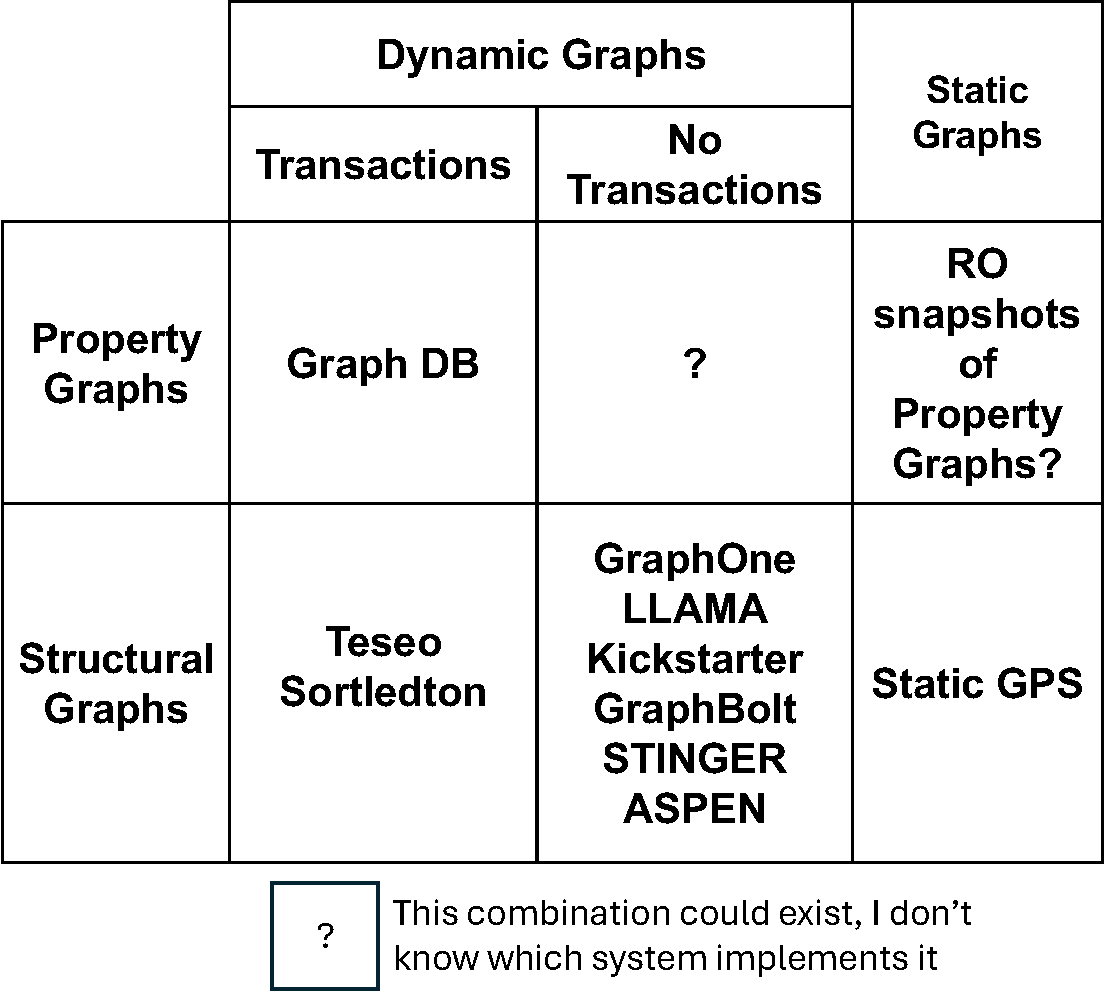
\includegraphics[scale=0.45]{fig/background/design_grid.pdf}
  \caption{Distillation of the design space of graph data management systems. Please refer to~\autoref{design:dynamic_structural} for an explanation of how the systems listed in the dynamic but not transactional category differ from one another.}
    \label{fig:distilled_design_space}
\end{figure*}
The main takeaway from this grid is that graph databases are the most general class of graph data management systems: they manage property graphs (of which structural graphs are a subset), support dynamic mutations, and provide transactional guarantees.
All the other categories are specialized to handle a subset of these features.
Each of those systems works well for the use cases for which it was designed, but none is as general as a graph database.
\project{} is designed to be a general-purpose graph data management system that can flexibly support all the specialized use cases depicted in this grid \emph{without moving data or sacrificing performance}.
